% FAM Architecture Diagram — NeurIPS 2026
% Compile: pdflatex fig_architecture.tex
%
% FIGURE DESIGN
% Message: "FAM pretrains a causal encoder via horizon-aware representation
%           prediction, then finetunes only the predictor+head to produce
%           monotonic event probability surfaces via discrete hazard CDF."
% Type: Architecture diagram (two-part: pretraining + finetuning)
% Layout: Two rows separated by dashed line. Left-to-right flow.
%         Tokenizer compressed. Encoder is central. Predictor+head on right.
% Colors: Blue=encoder, Green=target encoder, Orange=predictor, Red=event head
% Size: NeurIPS single column (5.5in / ~14cm)
%
\documentclass[border=3pt,tikz]{standalone}
\usepackage{tikz}
\usepackage{xcolor}
\usepackage{mathptmx}
\usepackage{amsmath,amssymb}

\usetikzlibrary{
  arrows.meta,
  positioning,
  shapes.geometric,
  fit,
  backgrounds,
  calc,
  decorations.pathreplacing,
}

% --- Palette (Okabe-Ito) ---
\definecolor{okBlue}{HTML}{0072B2}
\definecolor{okOrange}{HTML}{E69F00}
\definecolor{okGreen}{HTML}{009E73}
\definecolor{okVermillion}{HTML}{D55E00}
\definecolor{okSkyBlue}{HTML}{56B4E9}
\definecolor{frozenGray}{HTML}{999999}
\definecolor{grayFill}{HTML}{EFEFEF}

% --- Reusable styles ---
\tikzset{
  blk/.style={
    draw=#1!70!black, fill=#1!10, rectangle, rounded corners=1.5pt,
    minimum height=0.5cm, minimum width=1.2cm,
    font=\sffamily\fontsize{6.5}{8}\selectfont, align=center, line width=0.4pt,
  },
  blk/.default=okBlue,
  frozen/.style={
    draw=frozenGray, fill=grayFill, rectangle, rounded corners=1.5pt,
    minimum height=0.5cm, minimum width=1.2cm,
    font=\sffamily\fontsize{6.5}{8}\selectfont, align=center, line width=0.4pt,
    text=frozenGray!60!black,
  },
  emb/.style={
    draw=#1!70!black, fill=#1!18, circle,
    minimum size=0.42cm, inner sep=0pt,
    font=\fontsize{6}{7}\selectfont, align=center, line width=0.4pt,
  },
  emb/.default=okBlue,
  arr/.style={
    -{Stealth[length=1.5mm, width=1.1mm]}, line width=0.4pt, black!65,
  },
  arrd/.style={
    -{Stealth[length=1.5mm, width=1.1mm]}, line width=0.4pt, dashed, black!45,
  },
  inp/.style={
    draw=black!50, fill=black!4, rectangle,
    minimum height=0.5cm, minimum width=0.8cm,
    font=\sffamily\fontsize{5.5}{7}\selectfont, align=center, line width=0.3pt,
  },
  lbl/.style={font=\sffamily\fontsize{6}{7}\selectfont, black!75},
  lbls/.style={font=\sffamily\fontsize{5.5}{6.5}\selectfont, black!55},
  sechd/.style={font=\sffamily\bfseries\fontsize{7.5}{9}\selectfont, black!85},
  lossn/.style={
    draw=okVermillion!70!black, fill=okVermillion!10, rectangle,
    rounded corners=1.5pt, minimum height=0.42cm, minimum width=0.55cm,
    font=\sffamily\fontsize{6.5}{8}\selectfont, align=center, line width=0.4pt,
  },
  gbox/.style={
    draw=#1!30, fill=#1!3, rounded corners=3pt, inner sep=3.5pt,
    line width=0.3pt,
  },
}

\begin{document}
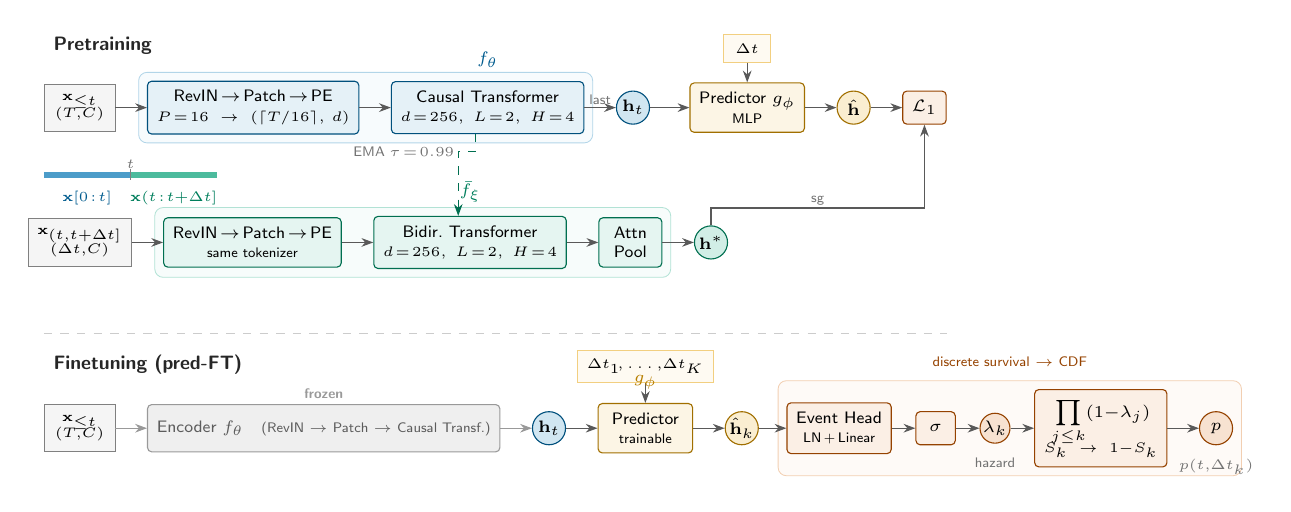
\begin{tikzpicture}[node distance=4mm and 5mm]

% =====================================================================
%  PRETRAINING — CONTEXT PATH
% =====================================================================

\node[sechd] (pt_lbl) at (0, 0) {Pretraining};

% Input
\node[inp, below=2.5mm of pt_lbl.south west, anchor=north west,
      minimum width=0.9cm, minimum height=0.6cm]
  (xctx) {$\mathbf{x}_{\leq t}$\\[-1pt]{\fontsize{4.5}{5.5}\selectfont$(T,\!C)$}};

% Tokenizer (compact: RevIN + Patch + PE in one block)
\node[blk=okBlue, right=4mm of xctx, minimum width=1.9cm]
  (tok_ctx) {RevIN $\!\to\!$ Patch $\!\to\!$ PE\\[-1pt]
  {\fontsize{4.5}{5.5}\selectfont$P\!=\!16\;\to\;(\lceil T/16\rceil,\,d)$}};

% Causal Transformer
\node[blk=okBlue, right=4mm of tok_ctx, minimum width=1.8cm]
  (enc) {Causal Transformer\\[-1pt]
  {\fontsize{4.5}{5.5}\selectfont$d\!=\!256,\; L\!=\!2,\; H\!=\!4$}};

% h_t
\node[emb=okBlue, right=4mm of enc] (ht) {$\mathbf{h}_t$};

% Predictor
\node[blk=okOrange, right=5mm of ht, minimum width=1.3cm]
  (pred) {Predictor $g_\phi$\\[-1pt]{\fontsize{4.5}{5.5}\selectfont MLP}};

% Delta-t input
\node[inp, above=2.5mm of pred, minimum width=0.6cm, minimum height=0.35cm,
      draw=okOrange!50, fill=okOrange!5]
  (dt_in) {$\Delta t$};

% h-hat
\node[emb=okOrange, right=4mm of pred] (hhat) {$\hat{\mathbf{h}}$};

% Loss
\node[lossn, right=4mm of hhat] (loss) {$\mathcal{L}_1$};

% Context path arrows
\draw[arr] (xctx) -- (tok_ctx);
\draw[arr] (tok_ctx) -- (enc);
\draw[arr] (enc) -- node[lbls, above, inner sep=1pt] {last} (ht);
\draw[arr] (ht) -- (pred);
\draw[arr] (dt_in) -- (pred);
\draw[arr] (pred) -- (hhat);
\draw[arr] (hhat) -- (loss);

% Encoder label
\node[lbl, text=okBlue!80!black, above=0.5mm of enc.north] {$f_\theta$};

% =====================================================================
%  PRETRAINING — TARGET PATH
% =====================================================================

% Target input (below context input)
\node[inp, below=11mm of xctx, minimum width=0.9cm, minimum height=0.6cm]
  (xtgt) {$\mathbf{x}_{(t,t{+}\Delta t]}$\\[-1pt]
  {\fontsize{4.5}{5.5}\selectfont$(\Delta t,\!C)$}};

% Tokenizer
\node[blk=okGreen, right=4mm of xtgt, minimum width=1.9cm]
  (tok_tgt) {RevIN $\!\to\!$ Patch $\!\to\!$ PE\\[-1pt]
  {\fontsize{4.5}{5.5}\selectfont same tokenizer}};

% Bidirectional Transformer
\node[blk=okGreen, right=4mm of tok_tgt, minimum width=1.8cm]
  (tgt_enc) {Bidir.\ Transformer\\[-1pt]
  {\fontsize{4.5}{5.5}\selectfont$d\!=\!256,\; L\!=\!2,\; H\!=\!4$}};

% Attention pool
\node[blk=okGreen, right=4mm of tgt_enc, minimum width=0.8cm]
  (apool) {Attn\\[-1pt]Pool};

% h*
\node[emb=okGreen, right=4mm of apool] (hstar) {$\mathbf{h}^*$};

% Target path arrows
\draw[arr] (xtgt) -- (tok_tgt);
\draw[arr] (tok_tgt) -- (tgt_enc);
\draw[arr] (tgt_enc) -- (apool);
\draw[arr] (apool) -- (hstar);

% Target encoder label
\node[lbl, text=okGreen!80!black, above=0.5mm of tgt_enc.north] {$\bar{f}_\xi$};

% h* to loss: route upward
\draw[arr] (hstar.north) -- ++(0, 0.22)
  -| node[lbls, pos=0.25, above, inner sep=1pt] {sg} (loss.south);

% --- EMA arrow (encoder -> target encoder) ---
\draw[arrd, okGreen!70!black]
  ($(enc.south) + (-0.15, 0)$) -- ++(0, -0.22)
  -| node[lbls, pos=0.3, left=0.5pt] {EMA $\tau\!=\!0.99$}
  ($(tgt_enc.north) + (-0.15, 0)$);

% --- Interval annotations ---
% Small timeline showing context | target (no gap)
\coordinate (tl_start) at ($(xctx.south west) + (0, -0.55)$);
\draw[black!40, line width=0.3pt]
  (tl_start) -- ++(2.2, 0);
\draw[okBlue!70, line width=2pt]
  (tl_start) -- ++(1.1, 0)
  node[lbls, midway, below=1.5pt, text=okBlue!80!black] {$\mathbf{x}[0\!:\!t]$};
\draw[okGreen!70, line width=2pt]
  ($(tl_start) + (1.1, 0)$) -- ++(1.1, 0)
  node[lbls, midway, below=1.5pt, text=okGreen!80!black] {$\mathbf{x}(t\!:\!t{+}\Delta t]$};
% Tick at boundary
\draw[black!50, line width=0.3pt]
  ($(tl_start) + (1.1, 0.07)$) -- ++(0, -0.14)
  node[lbls, above=1pt] {$t$};
% (removed "no gap" annotation)

% =====================================================================
%  DASHED SEPARATOR
% =====================================================================

\coordinate (sep_y) at ($(xtgt.south) + (0, -0.85)$);
\draw[draw=black!20, dashed, line width=0.35pt]
  (pt_lbl.west |- sep_y) -- (loss.east |- sep_y);

% =====================================================================
%  FINETUNING (pred-FT)
% =====================================================================

\node[sechd, anchor=west] (ft_lbl)
  at (pt_lbl.west |- sep_y) [yshift=-4mm] {Finetuning (pred-FT)};

% Input
\node[inp, below=2.5mm of ft_lbl.south west, anchor=north west,
      minimum width=0.9cm, minimum height=0.6cm]
  (ft_x) {$\mathbf{x}_{\leq t}$\\[-1pt]{\fontsize{4.5}{5.5}\selectfont$(T,\!C)$}};

% Frozen encoder (single compressed block)
\node[frozen, right=4mm of ft_x, minimum width=3.2cm, minimum height=0.6cm]
  (ft_enc) {Encoder $f_\theta$\quad
  {\fontsize{4.5}{5.5}\selectfont(RevIN $\to$ Patch $\to$ Causal Transf.)}};

% Frozen label
\node[lbls, text=frozenGray, above=-0.5mm of ft_enc.north, anchor=south]
  {\textbf{frozen}};

% h_t
\node[emb=okBlue, right=4mm of ft_enc] (ft_ht) {$\mathbf{h}_t$};

% Predictor (trainable)
\node[blk=okOrange, right=4mm of ft_ht, minimum width=1.2cm]
  (ft_pred) {Predictor\\[-1pt]{\fontsize{4.5}{5.5}\selectfont trainable}};

% Horizons input
\node[inp, above=2.5mm of ft_pred, minimum width=1.0cm, minimum height=0.35cm,
      draw=okOrange!50, fill=okOrange!5]
  (ft_dt) {$\Delta t_1\!,\ldots,\!\Delta t_K$};

% h-hat at each horizon
\node[emb=okOrange, right=4mm of ft_pred] (ft_hk) {$\hat{\mathbf{h}}_k$};

% Event head
\node[blk=okVermillion, right=3.5mm of ft_hk, minimum width=1.1cm]
  (ehead) {Event Head\\[-1pt]{\fontsize{4.5}{5.5}\selectfont LN\,+\,Linear}};

% Sigma
\node[blk=okVermillion, right=3mm of ehead, minimum width=0.5cm, minimum height=0.42cm]
  (sig) {$\sigma$};

% Lambda
\node[emb=okVermillion, right=3mm of sig, minimum size=0.38cm]
  (lam) {$\lambda_k$};

% Survival CDF
\node[blk=okVermillion, right=3mm of lam, minimum width=1.5cm]
  (cdf) {${\displaystyle\prod_{j\leq k}}(1{-}\lambda_j)$\\[-2pt]
  {\fontsize{4.5}{5.5}\selectfont$S_k \;\to\; 1{-}S_k$}};

% Output surface
\node[emb=okVermillion, right=4mm of cdf, minimum size=0.42cm]
  (pout) {$p$};

% Finetuning arrows
\draw[arr, frozenGray] (ft_x) -- (ft_enc);
\draw[arr, frozenGray] (ft_enc) -- (ft_ht);
\draw[arr] (ft_ht) -- (ft_pred);
\draw[arr] (ft_dt) -- (ft_pred);
\draw[arr] (ft_pred) -- (ft_hk);
\draw[arr] (ft_hk) -- (ehead);
\draw[arr] (ehead) -- (sig);
\draw[arr] (sig) -- (lam);
\draw[arr] (lam) -- (cdf);
\draw[arr] (cdf) -- (pout);

% Annotations
\node[lbls, below=0.5mm of lam.south, text width=1.2cm, align=center]
  {hazard};
\node[lbls, below=0.5mm of pout.south] {$p(t,\!\Delta t_k)$};

\node[lbl, text=okOrange!80!black, above=0.5mm of ft_pred.north] {$g_\phi$};

% =====================================================================
%  GROUP BOXES (background)
% =====================================================================

\begin{scope}[on background layer]
  % Context encoder group
  \node[gbox=okBlue, fit=(tok_ctx)(enc), inner sep=3pt] {};
  % Target encoder group
  \node[gbox=okGreen, fit=(tok_tgt)(tgt_enc)(apool), inner sep=3pt] {};
  % Hazard-CDF chain
  \node[gbox=okVermillion, fit=(ehead)(sig)(lam)(cdf)(pout), inner sep=3pt] (cdf_group) {};
\end{scope}

% CDF group label
\node[lbls, text=okVermillion!70!black, above=0.5mm of cdf_group.north]
  {discrete survival $\to$ CDF};

\end{tikzpicture}
\end{document}
